% 
%  backgroundChapter.tex
%  ThesisISEL
%  
%  Created by Sana on 2023/01/28.
%

\chapter{Background}
\label{cha:background_chapter}

This section offers essential background information to comprehend the scope of our work. We commence by introducing vulnerability discovery, presenting foundational concepts within the context of machine learning, static analysis, Abstract Syntax Trees (AST), and Control Flow Graphs (CFG), elaborating on these aspects in further detail. Subsequently, we present an overview of the potential vulnerabilities that will be addressed in our study.


% ================
% = Discovering vulnerabilities =
% ================
\section{Discovering vulnerabilities} % (fold)
\label{sec:	Discovering_vulnerabilities}

European Union Agency for Cybersecurity (ENISA) \cite{Wikipedia_ENISA} defines vulnerability in \cite{ENISA} as: \textit{``The existence of a weakness, design, or implementation error that can lead to an unexpected, undesirable event compromising the security of the computer system, network, application, or protocol involved''}. Likewise, they are described as \textit{``A weakness of an asset or group of assets that can be exploited by one or more threats, where an asset is anything that has value to the organization, its business operations, and their continuity, including information resources that support the organization's mission''} in the norm ISO/IEC 27005:2008 \cite{ISO_27005}. \\

Three key factors can essentially lead to a software vulnerability:
\begin{itemize}
\item  \textbf{Design or specification phase}: During the design phase, important architectural decisions are made, including the choice of programming languages, frameworks, and libraries. Poor choices or inadequate consideration of security requirements at this stage can lead to vulnerabilities. For example, selecting a framework with known security issues or not properly isolating components can introduce vulnerabilities.

\item \textbf{Implementation phase}: The implementation phase of software development is a critical stage where vulnerabilities can either be introduced or mitigated. Secure coding practices, adherence to secure coding standards, thorough testing, and attention to security details are essential to minimize the risk of vulnerabilities in the final product. Regularly updating and patching software components is also crucial for ongoing security.

\item \textbf{The deployment phase}: The deployment phase of software development can have a significant impact on software vulnerability. This phase involves the installation, configuration, and setup of the software in its intended environment. Properly configuring security settings, access controls, encryption, and monitoring is essential to ensure that the software remains secure in its operational environment. Additionally, ongoing maintenance and patch management are crucial for long-term security.

\end{itemize}

There are multiple techniques employed for vulnerability discovery, which can be categorized into static analysis, involving the processing of code without execution; dynamic analysis, where code behavior is analyzed during execution; and hybrid techniques that combine elements of both. These three methods are described in the subsequent sections, preceding the presentation of the fundamental concepts of Machine Learning approaches, along with a discussion of certain vulnerabilities in our case study.


% section Discovering_vulnerabilities (end)


% ================
% = Static analysis =
% ================
\section{Static analysis} % (fold)
\label{sec:	Static_analysis}

In static code analysis, a program is examined structurally without actual execution. In this approach, potential vulnerabilities are identified \cite{5066568} through techniques like \textit{taint analysis} and \textit{data flow analysis}. Static analysis provide support for code reviews by highlighting potential vulnerabilities and security weaknesses. Developers can review and address these issues before the code is committed, reducing the likelihood of vulnerabilities making their way into production. Static analysis tools can be used to recognize patterns and coding practices that are indicative of common vulnerabilities. For example, they can identify instances of SQL injection, cross-site scripting (XSS), buffer overflows, and other security issues based on known coding patterns. Static code analysis tools automatically scan the source code of an application, examining each line and component for potential vulnerabilities. This automation makes it possible to analyze large and complex codebases efficiently. This method holds certain advantages, including enabling faster inspection cycles for fixes, and it is relatively efficient. However, it also has limitations. For instance, it cannot uncover vulnerabilities introduced in the runtime environment \cite{5066568}. Additionally, due to imperfect models, static analysis often generates false positives, requiring human intervention.\\

Within static analysis, various approaches can be used, including rule matching, pointer analysis, taint analysis, lexical analysis, model checking, data-flow analysis, and dependency analysis \cite{Mukesh_Kumar_2015, Bingchang_2012}. The concept behind taint analysis is that any variable that can be altered by the user, either directly or indirectly, should be regarded as tainted, as it holds the potential to develop into a security vulnerability. Variables that stem from tainted variables also inherit the tainted status.\\ 

Lexical analysis involves scanning the source code to identify patterns or abstract syntax. Overall, lexical analysis is a critical step in the compilation process, as it transforms human-readable source code into a format that can be processed by the subsequent stages of a compiler or interpreter. This process simplifies the task of understanding and manipulating the code's structure and semantics.\\

Data flow analysis involves examining how data values are manipulated, transformed, and transferred between variables and functions throughout the code.\\

The first static analysis tools that were introduced were basic program checkers \cite{JViega_2000}. These tools were not highly advanced and often consisted of simple commands like grep or find, relying on a lexical analysis approach. There exists an extensive list of vulnerability scanners employed in practical settings, including tools like PScan \cite{PScan}, Microsoft PREfast \cite{Larus_2004}, and JSLint \cite{JSLint}, which enforce sound programming practices. These tools are invaluable, particularly in development environments. However, they fall short when it comes to identifying more intricate and nuanced vulnerabilities. These tools were swiftly succeeded by numerous commercial counterparts designed for various programming languages, all aiming to accomplish automated source code reviews.

The precision of static analysis tools is evaluated through the calculation of the false positive rate, and it is constrained by computational limitations as well as the rate of false positives. The significant occurrence of false positives in numerous tools poses a considerable challenge \cite{Kui_Liu2018}, as these misclassifications require developers to invest substantial time in verifying each one, thereby complicating the identification of actual issues.


% section Static_analysis(end)


% ================
% = Dynamic and hybrid analysis =
% ================
\section{Dynamic and hybrid analysis} % (fold)
\label{sec:	Dynamic_hybrid_analysis}

Another technique that can be employed to discover vulnerabilities is dynamic analysis, wherein computer software is analyzed on a real or virtual processor \cite{5066568} through the execution and monitoring of programs during runtime. Dynamic analysis tools try to execute the program using various inputs and monitor its behavior, while static analysis tools aim to construct a model of the program's state to identify potential behaviors through a logical process.

Dynamic analysis approaches can be divided into two main categories: concrete and symbolic execution. Noteworthy applications of dynamic concrete execution include: fuzzing \cite{Godefroid_2012, Vijay_Ganesh2009}, wherein malformed input is provided to provoke crashes; and taint-based fuzzing \cite{Newsome2005, Sofia_Bekrar2012}, which assesses how the program handles input to determine which portions of the input require modification in subsequent runs.

Dynamic analysis offers certain advantages, including the ability to identify vulnerabilities during runtime and the capability to analyze applications that lack access to the actual code. However, it also presents limitations, such as the absence of adequately trained professionals to conduct dynamic code analysis. Additionally, tracing the vulnerability back to the precise location in the code is more challenging \cite{5066568}.

The major issue with Dynamic analysis is that it demands significantly more computational time and resources, and is often infeasible in many scenarios, particularly when evaluating larger software or collections of software.\\

Hybrid analysis combines both static and dynamic analysis techniques to enhance the effectiveness of vulnerability detection in code. This approach leverages the strengths of both methods to overcome their individual limitations. During hybrid analysis, the code is subjected to both static analysis, which involves examining the code's structure without execution, and dynamic analysis, which involves executing and monitoring the code in a runtime environment.\\

The goal of hybrid analysis is to achieve a more comprehensive and accurate assessment of the code's security posture. Static analysis helps identify potential vulnerabilities by analyzing the code's structure, logic, and potential patterns of misuse. Dynamic analysis, on the other hand, simulates real-world runtime scenarios, which can help uncover vulnerabilities that may only manifest during execution.\\

By combining these approaches, hybrid analysis aims to achieve a higher level of accuracy in identifying vulnerabilities, reduce false positives and negatives, and provide a more complete understanding of the code's security vulnerabilities. This approach is especially valuable when dealing with complex and large-scale software applications where relying solely on static or dynamic analysis may not provide sufficient coverage.

% section Dynamic_hybrid_analysis(end)



% ================
% = Representing source code =
% ================
\section{Representing source code} % (fold)
\label{sec: Representig_source_code}

There are different approaches available for preprocessing code and representing it in a suitable format when applying machine learning to source code. The upcoming sections will describe several commonly employed techniques that are frequently utilized in research studies, and as a result, will be referenced throughout this work.


% section Representing_source_code(end)


% ================
% = Abstract syntax trees (AST) =
% ================
\subsection{Abstract syntax trees (AST)} % (fold)
\label{sec: Abstract_syntax_trees}

An Abstract Syntax Tree (\gls{ast}) is a tree-based data structure that excellently captures the syntactic arrangement of the source code. Each node within this tree corresponds to a specific construct found within the source code. This structure offers a hierarchical depiction of the source code's composition, as highlighted by Liu \cite{Kui_Liu2018}.

An \gls{ast} commonly emerges as the outcome of the syntax analysis phase within a compiler. Frequently, it operates as an intermediary representation of the program across various stages essential for the compiler's functionality. Notably, the \gls{ast} substantially influences the ultimate output produced by the compiler, as noted by Rahul Khinchi \cite{rahulkhinchi7}.\\ 

\begin{figure}[ht]
	\centering
	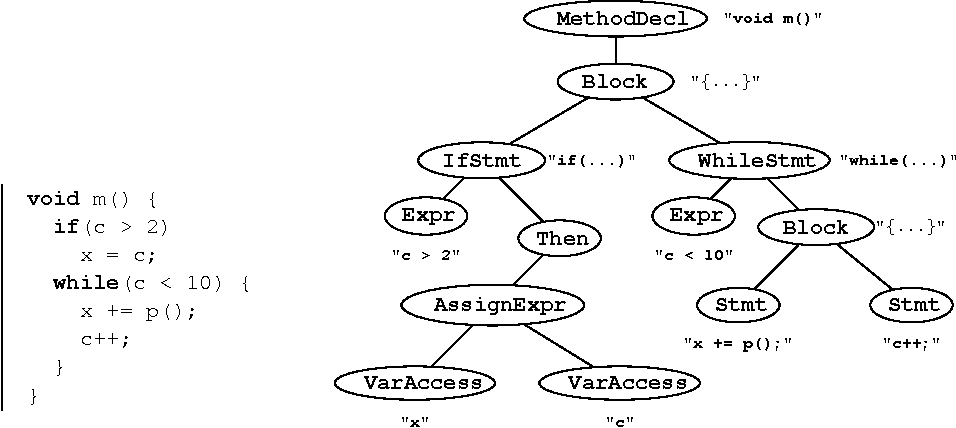
\includegraphics[width=0.90\textwidth]{AST}
	  \caption{Sample Java method and its abstract syntax tree}
  \label{fig:java_ast}
\end{figure}


Figure \ref{fig:java_ast} illustrates an example of an abstract syntax tree for a Java method. Each node is depicted as a construct that occurs within the source code.    

%https://www.semanticscholar.org/paper/Extensible-%intraprocedural-flow-analysis-at-the-S%C3%B6derberg-%Ekman/7a8251f687d09a661e77bc8a4e409736ea61ede9/figure/0

To build an Abstract Syntax Tree (\gls{ast}), a specific program analysis involves two fundamental operations: lexical analysis and syntax analysis. These processes are described as follows: \textbf{lexical} and \textbf{syntax analysis}.

\begin{enumerate}
\item \textbf{Lexical Analysis (Lexing)} involves transforming the source code of a program into a sequence of tokens (lexemes). Each token is a data structure that signifies a specific type, such as identifiers, keywords, and operators. A program dedicated to performing lexical analysis is typically referred to as a lexer, tokenizer, or scanner. Essentially, a token can be understood as a string endowed with a recognized significance. It is structured as a pair comprising a token name and an optional token value, as outlined by Alfred \cite{Alfred_V2007}.;
\item \textbf{Syntax Analysis (Parsing)} entails examining a string of symbols in accordance with the regulations of a formal grammar known as Context-Free Grammar. A program designed for conducting syntax analysis is typically termed a parser, as noted by Douglas Thain \cite{Douglas_Thain}. 
\end{enumerate}

Yamaguchi et al. \cite{Fabian_Markus_Konrad2023} translated \gls{ast} graphs into vectors and subsequently applied a natural language processing technique known as latent semantic analysis to identify correlations between established vulnerabilities and possible vulnerabilities present in the code. Through this approach, they successfully identified novel vulnerabilities within multiple open-source projects \cite{Fabian_Markus_Konrad2023}.

The applications of \gls{ast} are diverse, often finding utility in the realm of static code analysis.

% subsection Abstract_syntax_trees(end)

% ================
% = Control Flow Graph (CFG) =
% ================
\subsection{Control Flow Graph (CFG)} % (fold)
\label{sec: Control_Flow_Graph}

A \gls{cfg} corresponds to a graphical depiction of control flow or computational sequences during program execution. It adopts the structure of a directed graph, where nodes embody basic blocks and edges symbolize potential transitions of control flow from one basic block to another. Within a \gls{cfg}, in addition to the basic blocks, two specifically designated blocks are present: the \textit{entry} and \textit{exit} blocks. The entry block allows the control flow to enter into the graph, likewise the control flow leaves through the exit block. This is how a control flow graph can depict how different program units or applications process information between different ends in the context of the system \cite{Kronjee2018}.

\begin{figure}[ht]
	\centering
	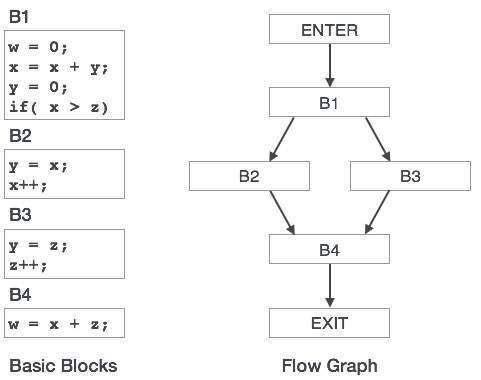
\includegraphics[width=\textwidth]{CFG}
	  \caption{Control Flow Graph example}
  \label{fig:CFG_EX}
\end{figure}

Figure \ref{fig:CFG_EX} depicts an example of a Control Flow Graph (\gls{cfg}). Block B1 represents an if statement and branches into two distinct blocks based on the condition (x > 5): B2 if the condition is true, or B3 otherwise.

A Control Flow Graph (\gls{cfg}) facilitates the identification of unreachable sections of code within a program, and it simplifies the detection of syntactic structures such as loops within the graph's structure.

Control flow graph techniques find significant application in data-flow analysis and compiler-related tasks. The forthcoming sections will delve into several techniques employed within data-flow analysis, namely Reaching Definitions, Use-Definition chains, and Taint Analysis. These techniques will also be employed in our own work.

% subsection Control_Flow_Graph (end)

% ================
% = Data Flow Analysis =
% ================
\section{Data Flow Analysis} % (fold)
\label{sec: Data_Flow_Analysis}

The subsequent sections discusses techniques used in software analysis and the acquisition of information regarding potential values computed at different junctures within the program. These techniques will consequently find application in the research.

% ================
% = Reaching definitions analysis =
% ================
\subsection{Reaching definitions analysis} % (fold)
\label{sec:Reaching_definitions_analysis}

Reaching definitions analysis \cite{Kronjee2018} constitutes a component of the data-flow analysis approach. Within this method, the definitions that could potentially reach (or be assigned to) a specific point within the code are ascertained. A definition \textbf{d} of a variable \textbf{v} denotes a statement that allocates a value to the variable \textbf{v}. A definition \textbf{d} reaches point \textbf{p} if a pathway exists from the location immediately following \textbf{d} to \textbf{p}, wherein \textbf{d} remains unaltered (not \textit{killed}) along that pathway. 

For example, within the following code blocks:
\[B1: a=3\] 
\[B3: a=4\]
\[B4: x=a\]


A pathway exists between B1 and B4 through B3, signifying that the definition of variable "a" in B1 does not extend to B4 due to the intervening influence of B3, which effectively terminates its reach. A definition of any variable is considered "killed" when a re-assignment occurs between two points along the path.

To compute reaching definitions, IN-OUT Analysis is conducted as described by Alfred \cite{Alfred_V2007}. For each basic block \textbf{B} in a \gls{cfg}, the following sets are established: \(GEN[B]\) represents all definitions generated in block B; \(KILL[B]\) represents other definitions that are overlaped (killed) the definitions generated in block B; \(IN[B]\) are all definitions of the previous blocks, i.e. it turns out to be the union of all \(OUT[p]\) for each predecessor \textbf{p} of block B \(IN[B] = \cup OUT[p]\); \(OUT[B]\) are all definitions generated in block B and all definition that have not been "Crushed" in block B. That is, OUT[B] is the union of all definitions in \(GEN[B]\) with those that are in \(IN[B]\) and not in \(KILL[B]\), i.e, $ OUT[B] = GEN[B] \cup  \left(IN[B] - KILL[B]\right) $.


\begin{figure}[ht]
	\centering
	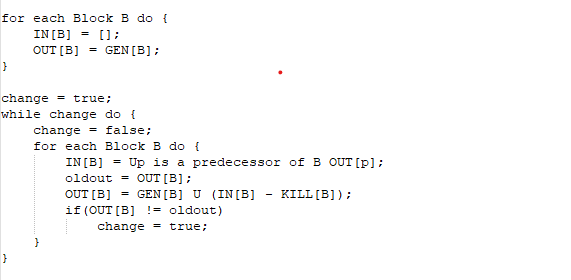
\includegraphics[width=\textwidth]{RDAlgorithm2}
	  \caption{Algorithm for Computing Reaching Definitions}
  \label{fig:RD_algorithm}
\end{figure}

Figure \ref{fig:RD_algorithm} presents the reaching definitions algorithm, adapted from the book "Compilers: Principles, Techniques, and Tools" \cite{Alfred_V2007}, tailored to our specific objectives.

The objective is to ascertain, for every point in the program, the assignments that have been executed and persist without being overwritten when execution reaches that specific point via a given pathway. Reaching definitions is used to determine \textit{use-def chains}, which in turn help identify instances of uninitialized or null variables being utilized.

% subsection Reaching definitions analysis (end)

% ================
% = Use-definition Analysis =
% ================
\subsection{Use-definition (UD) Analysis} % (fold)
\label{sec:Use_definition_Analysis}

A \gls{ud} chain consists of a use of a variable, and all the definitions of that variable that can reach that use without any other intervening definitions. They are constructed based on IN set for a particular definition \cite{Kronjee2018}. Null pointer deference and Command injection vulnerabilities are typically due to the use of potentially vulnerable functions and a lack of sanitization. This is the reason why we will use use-definition chain as well.\\



%\subsection{Computing ud-chains} % (fold)
%\label{sub: Computing_ud_chains}

{\Large Computing ud-chains} \\

As previously mentioned, we can  compute  ud-chains  from  the reaching definitions  information. If  a use  of a variable \textbf{A} is preceded in its block  by  a definition  of \textbf{A}, then  only  the last  definition of \textbf{A}  in the block  prior to this use  reaches  the use. Thus the list or ud-chain for this use  consists of only this one definition. If a use of \textbf{A} is preceded  in its block \textbf{B} by no definition of \textbf{A}, then the ud-chain for this use consists of all definitions of \textbf{A} in \(IN[B]\).

Let U be the statement in question using A:

\begin{enumerate}
\item If there are definitions of A within block B prior to statement U, then the last such definition is the only definition of A reaching U\\

Block B1:\\
\(d1: A = 2\)\\ 
\(d2: B = A + 1\)\\

Block B2:\\
\(d3: A = 1\)\\

Then: <d2, A > = \{d1\} (d1 is the definition of A in d2 )

\item If there are no definition of A within block B prior to U, then the definitions of A reaching U are these definitions of A that are in IN[B]\\

Block B1:\\
\(d1: A = 5\)\\ 

Lets suppose that IN[B1] = \{d1, d2, d3, d4, d5\} and the definition of A in set IN[B1] are \{d2, d5\}, then:
<d1, A> = \{d2, d5\}

\end{enumerate}

% subsection Computing ud-chains (end)

% section Use-definition Analysis (end)

% ================
% = Taint analysis =
% ================
\subsection{Taint analysis} % (fold)
\label{sec: Taint_analysis}

Taint analysis is a methodology employed to inject potentially harmful data into a target program, subsequently scrutinizing the trajectory of data propagation to assess program security. This technique was initially introduced in 1998 \cite{Ren_2020}, garnering continuous interest from researchers since its inception. Taint analysis has found extensive application in the detection of information leakage, identification of vulnerabilities, reverse engineering, and other related fields.

The taint analysis process is generally structured into three sequential stages \cite{REN_Yuzhu2019}: taint source identification, taint propagation analysis, and taint convergence point detection. Taint sources denote the locations within an application where access to potentially contaminated data occurs. Among these stages, taint propagation analysis stands as the pivotal component of taint analysis methodology. The accuracy of taint propagation analysis is significantly influenced by the taint propagation strategy model.

There are two problems with taint analysis techniques, namely over-taining and under-taining as highlighted by \cite{REN_Yuzhu2019}. Over-taining means that data variables with no dependence on the taint source are marked as taint in the process of taint propagation, that is, false positives are generated. Under-taining is that data variables with dependence on the taint source are not marked as taint in the process of taint propagation, that is, false negatives are generated.

Taint analysis identifies every source of user data, encompassing inputs, headers, and subsequent data flows. It traces each fragment of data throughout the system to ensure its proper sanitization prior to utilization. For instance, an application could be susceptible to command injections if it employs unverified external data to execute a command line on the system.

% subsection Taint analysis (end)



% ================
% = Machine learning =
% ================
\section{Machine learning (\gls{ml})} % (fold)
\label{sec: Machine_learning}

This section focuses essentially on the techniques used in the development of our tool.\\

The pioneer of \gls{ml}, Arthur Samuel, defined \gls{ml} as a “field of study that gives computers the ability to learn without being explicitly programmed.” \gls{ml} focuses on classification and prediction, based on known properties previously learned from the training data. \gls{ml} algorithms need a goal (problem formulation) from the domain (e.g., dependent variable to predict). the system to learn from experience and form concepts from examples by extracting patterns from the raw data \cite{Goodfellow_et_al_2016}.

An \gls{ml} approach usually consists of two phases: training and testing. But sometimes, the following steps are performed:

\begin{itemize}
\item  Identifying class attributes (features) and classes from training data;
\item  Identifying a subset of the attributes necessary for classification;
\item  Learning the model using training data;
\item  Using the trained model to classify the unknown data.
\end{itemize}

Any Machine Learning method is likely subjective to overfitting, i.e. certain particular features present in a training set which damage the performance for new and not observed examples. This behavior has consequence on error estimation over the training set (the result is overly optimistic). Therefore a separated set of not observed samples is required for an unbiased error estimation \cite{C_M_Bishop2006}. 

If we want to use error estimation for choosing the best set of hyperparameters (parameters of a model training algorithm defined prior to the learning process) we must use a validation set for this purpose and leave an unseen test set for the final unbiased error estimate. This means that we must split the available data in three parts: the training, validation and test sets.

In fact, for most \gls{ml} methods, there should be three phases, not two: training, validation, and testing. After the training is complete, there are usually several models available. To decide which one to use and have a good estimation of the error the third separate data set (the validation data set) should be used. The model that performs the best on the validation data should be the model used, and should not be fine-tuned depending on its accuracy on the test data set. Otherwise, the accuracy reported is optimistic and might not reflect the accuracy that would be obtained on another test set similar to but slightly different from the existing test set \cite{Anna_L2016}.

There are three main types of \gls{ml} approaches: \textbf{unsupervised}, \textbf{semi-supervised}, and \textbf{supervised}. In unsupervised learning problems, the main task is to find patterns, structures, or knowledge in unlabeled data. When a portion of the data is labeled during acquisition of the data or by human experts, the problem is called semi-supervised learning. The addition of the labeled data greatly helps to solve the problem. If the data are completely labeled, the problem is called supervised learning and generally the task is to find a function or model that explains the data \cite{Tom_M_Mitchell1997}.

Once a classification model is developed by using training and validation data, the model can be stored so that it can be used later or on a different data.\\

The model building is constituted by the following phases: 

\begin{itemize}
\item Understanding the business: Defining the Data mining problem performed by the project requirements;
\item  Understanding the data: Data collection and examination;
\item Preparing the data: All aspects of data preparation to reach the final dataset;
\item Modeling: Applying \gls{ml} methods and optimizing parameters to fit the best model;
\item Evaluation: Evaluating the method with appropriate metrics to verify if business goals are reached;
\item  Implementation: Varies from submitting a report to a full implementation of the data collection and modeling framework.
\end{itemize}

Before delving into the algorithms used to create classification models, it's important to grasp the metrics used to evaluate the performance of such models.\\

According to Somogyi Zolt, et al., in their 2021 book titled "Performance Evaluation of Machine Learning Models," the typical metrics employed in model evaluation are as follows \cite{Somogyi2021}:

\textbf{{\Large Confusion Matrix}} \\

In the field of machine learning, a confusion matrix is a table used to describe the performance of a classification model on a set of data for which the true values are known \cite{Somogyi2021}. It's a fundamental tool for understanding the accuracy and behavior of a classification algorithm. The confusion matrix presents the actual and predicted classifications in a tabular format, allowing you to analyze the true positive, true negative, false positive, and false negative predictions made by the model.

\begin{figure}[ht]
	\centering
	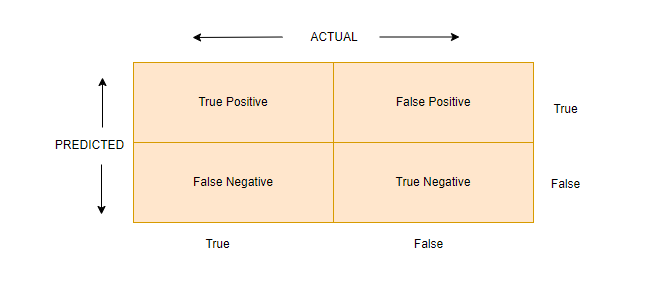
\includegraphics[width=0.95\textwidth]{ConfMatrix}
	  \caption{Confusion Matrix Example}
  \label{fig:ConfMatrix}
\end{figure}


\textbf{True Positives (TP)} are positive outcomes in which the model correctly predicts the positive class. In our case, it means: Predicting that the code is vulnerable, and it actually is.\\

\textbf{True Negatives (TN)} are negative outcomes in which the model correctly predicts the negative class. In our case, it means: Predicting that the code is vulnerable, but it is not.

\textbf{False Positives (FP)} are positive outcomes in which the model incorrectly predicts the positive class. In our case, it means: Predicting that the code is vulnerable, but it is not. \\

\textbf{False Negatives (FN)} are negative outcomes in which the model incorrectly predicts the negative class. For our case, it means: Predicting that the code is not vulnerable, but it is.\\

From the confusion matrix, various performance metrics can be derived, such as accuracy, precision, recall (sensitivity), specificity, F1-score, etc. These metrics provide a comprehensive understanding of how well the model is performing and can guide further optimization.

\textbf{Precision}\\

Is a performance metric that measures the accuracy of positive predictions made by a classification model. It focuses on the ratio of true positive predictions to the total number of instances predicted as positive (both true positives and false positives) \cite{Somogyi2021}.

Mathematically, precision is calculated as:

\begin{equation}\label{Precision_eq}Precision = \frac{TP}{TP + FP}\end{equation}

High precision indicates that the model makes fewer false positive errors, meaning that when it predicts a positive instance, it's more likely to be correct. However, optimizing for high precision might result in more false negatives (Type II errors), where positive instances are missed.

\textbf{Recall}\\

Also known as sensitivity or true positive rate, is a performance metric that measures the ability of a classification model to correctly identify all relevant instances of a particular class within a dataset. It is particularly important in cases where the consequences of missing positive instances (false negatives) are significant \cite{Somogyi2021}.

Mathematically, recall is calculated as:

\begin{equation}\label{Recall_eq}Recall = \frac{TP}{TP + FN}\end{equation}

Recall focuses on the ratio of true positive predictions to the total number of actual positive instances. A high recall indicates that the model is effectively identifying a large portion of the positive instances, which is important in scenarios where false negatives should be minimized, such as in our case, vulnerability detection.\\

\textbf{f1-score}\\

Is a performance metric that combines both precision and recall into a single value. It provides a balanced measure of a model's accuracy, considering both false positives (Type I errors) and false negatives (Type II errors) \cite{Somogyi2021}.

The F1-score is calculated as the harmonic mean of precision and recall:

\begin{equation}\label{F1_Score_eq}F1 Score = \frac{2*(Recall * Precision)}{(Recall + Precision)}\end{equation}

The F1-score ranges between 0 and 1, with a higher value indicating better model performance. It is particularly useful when dealing with imbalanced datasets or when the consequences of both false positives and false negatives are important.\\

\textbf{Area Under the ROC Curve (AUC-ROC)}\\

Measures the model's ability to discriminate between positive and negative classes across different threshold values. Higher AUC-ROC indicates better performance.

\textbf{ROC Curve}: The Receiver Operating Characteristic (ROC) curve is a graphical representation of a model's performance at different classification thresholds. It plots the True Positive Rate (Sensitivity) against the False Positive Rate (1 - Specificity) for different threshold values \cite{Somogyi2021}.\\

\textbf{AUC-ROC}: The Area Under the ROC Curve (AUC-ROC) is the area under the ROC curve. It ranges from 0 to 1, where higher values indicate better performance. A model with an AUC-ROC of 0.5 performs no better than random guessing, while an AUC-ROC of 1 indicates perfect discrimination between positive and negative classes \cite{Somogyi2021}.\\

AUC-ROC Interpretation:

\begin{itemize}
\item AUC-ROC values closer to 1 suggest that the model is better at correctly classifying instances and distinguishing between positive and negative classes.
\item AUC-ROC values around 0.5 indicate that the model's performance is similar to random guessing.
\item AUC-ROC values below 0.5 indicate that the model's predictions are worse than random guessing.
\end{itemize}

\textbf{Area Under the Precision-Recall Curve (AUC-PR)}\\

Is a performance metric used in machine learning to evaluate the quality of a binary classification model, especially when dealing with imbalanced datasets \cite{Somogyi2021}.


\textbf{Precision-Recall Curve}: The Precision-Recall curve is a graphical representation of a model's performance at different classification thresholds. It plots Precision (the ratio of true positive predictions to all positive predictions) against Recall (the ratio of true positive predictions to all actual positives) for different threshold values.

\textbf{AUC-PR: The Area Under the Precision-Recall Curve (AUC-PR)} is the area under the Precision-Recall curve. Similar to AUC-ROC, it ranges from 0 to 1, where higher values indicate better performance. A higher AUC-PR suggests that the model is better at achieving high precision while maintaining high recall.\\

Interpretation of AUC-PR:

\begin{itemize}
\item AUC-PR values closer to 1 suggest that the model has a good balance between precision and recall, effectively classifying positive instances while minimizing false positives.
\item AUC-PR values around 0.5 indicate that the model's performance is similar to random guessing.
\item AUC-PR values below 0.5 indicate that the model's predictions are worse than random guessing.
\end{itemize}

\textbf{Brier Score}\\

The Brier Score is a performance metric used in machine learning to assess the accuracy of probabilistic predictions made by a model, especially in binary classification tasks. It measures the mean squared difference between predicted probabilities and the actual outcomes \cite{Somogyi2021}.

The Brier Score ranges between 0 and 1, where lower values indicate better model performance. A Brier Score of 0 indicates perfect calibration, meaning that the predicted probabilities match the actual outcomes perfectly.\\

The following subsections will describe more about sophisticated learning methods that can be applied in vulnerability detection.


% section Machine_learning(end)

\subsection{Neural networks} % (fold)
\label{sub: Neural_networks}

A neural network consists of neurons, also called units or nodes.  They are inspired by the most complex object in the universe – the human brain.

The human brain consists of  “neurons” working in parallel and exchanging information through their connectors “synapses”.  These neurons sum up all information coming into them, and if the result is higher than the given potential called action potential, they send a pulse via axon to the next stage \cite{dspguide}.

A neural network also consists of simple computing units “artificial neurons,” and each unit is connected to the other units via weight connectors. Then, these units calculate the weighted sum of the coming inputs and find out the output using squashing function or activation function \cite{inbook}. Figure below shows the block diagram of neuron.

\begin{figure}[ht]
	\centering
	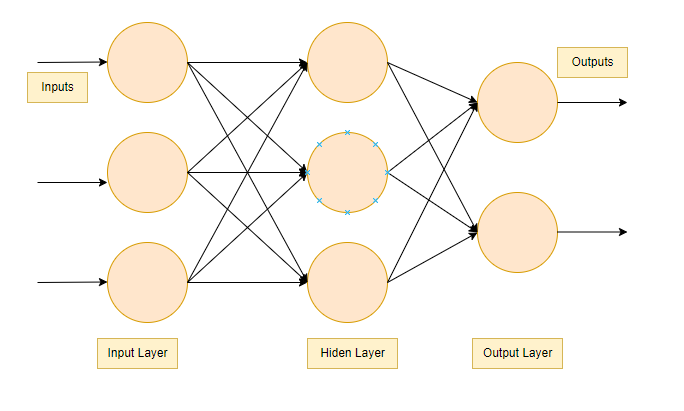
\includegraphics[width=0.95\textwidth]{Neural_Network}
	  \caption{Neural network diagram}
  \label{fig:Neural_Network}
\end{figure}

Neurons take input, process it, and pass it on to other neurons present in the multiple hidden layers \cite{inbook} of the network, till the processed output reaches the Output Layer.

Neural networks are used in many areas. They are predestined for applications in which there is little systematic solution knowledge and a large amount of sometimes imprecise input information must be processed to a concrete result \cite{article_Mijwil}. Areas of application can be speech recognition or image recognition. Neural networks can also create simulations and predictions for complex systems and relationships, such as in weather forecasting, medical diagnostics or business processes. Typical applications of neural networks are: Image recognition, Voice recognition, Pattern recognition and more.

Before a neural network can be used for the intended problem or task, it involve first be trained. Neural networks learn via supervised learning or Unsupervised learning. 

Supervised machine learning involves an input variable x and corresponding desired output variable y. The data will be presented in a form of couples (input, desired output), and then the learning algorithm will adapt the weights and biases depending on the error signal between the real output of network and the desired output.

Unsupervised machine learning has input data X and no corresponding output variables. A competitive learning rule is used. A neural network of two layers—an input layer and a competitive layer is used. The input layer receives the available data. The competitive layer consists of neurons that compete with each other (in accordance with a learning rule) for the “opportunity” to respond to features contained in the input data \cite{inbook}.

A neural network  is known as \textbf{a deep learning or deep neural network} when the newtwork has multiple hidden layers and multiple nodes in each hidden layer \cite{MOHAMMED_MUSTAPHA_MAMDOUH}. Deep learning is the development of deep learning algorithms that can be used to train and predict output from complex data.


 In Deep Learning, the word \textbf{“deep”} refers to the number of hidden layers i.e. depth of the neural network. Essentially, every neural network with more than three layers, that is, including the Input Layer and Output Layer can be considered a Deep Learning Model \cite{inbook_Singh}.

 It generally it takes more time to train deep learning model. They have higher accuracy than Neural Networks. It gives high performance compared to neural networks.

Deep learning models can be used in a variety of industries, including pattern recognition, speech recognition, natural language processing, and more.

% subsection Neural_networks (end)

\subsection{Decision Trees} % (fold)
\label{sub: Decision_Trees}

Decision trees \cite{J_Ross_Quinlan1994} are classifiers represented as trees where internal nodes are tests on individual features and leaves are classification decisions. Therefore internal nodes correspond to attributes and leaf nodes correspond to class labels.

Typically, a greedy heuristic search method is used to find a decision tree that correctly classifies the training data. The learning element is build as a tree by selecting the attribute that best splits the training set into their appropriate classes. It creates a node, branches, and children for the attribute and its values, removes the attribute from being considered further, and distributes the examples to the appropriate child node. This process repeats recursively until a node contains examples of the same class, at which point, it stores the class label \cite{J_Zico_Kolter2006}. The following tree algorithms are worthy of attention:  ID3, C4.5, CART, CHAID, and MARS \cite{Tom_M_Mitchell1997, Jerome_H_Friedman1991}.

One advantage of utilizing decision trees over other models is their exceptional interpretability and automatic feature selection. This enables thorough analysis to be conducted on decision trees.

Decision trees are especially well-suited for data characterized by discrete-valued features. Contemporary implementations involve trimming certain branches (those with unexpected information gain), which helps prevent overfitting. This technique is referred to as pruning. Pruning reduces the size of decision trees by eliminating segments of the tree that contribute little to the ability to classify observations.

\begin{figure}[ht]
	\centering
	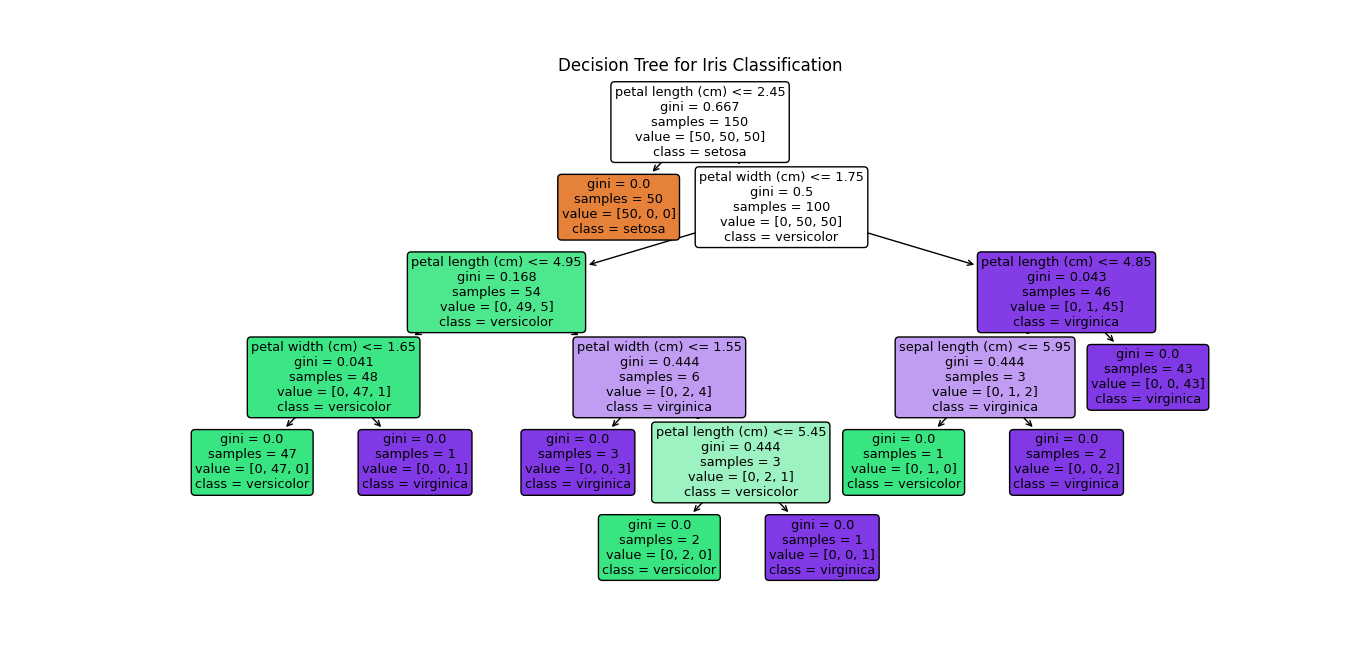
\includegraphics[width=0.95\textwidth]{DecisionTree}
	  \caption{Decision tree trained on the iris dataset}
  \label{fig:DecisionTree}
\end{figure}

The splitting process makes the method highly efficient. When training a decision tree classifier, the algorithm examines the features and determines which "splits" contain more information.

Figure \ref{fig:DecisionTree} illustrates a decision tree trained on a training set of the Iris dataset. At each step, the outcome of the comparison determines whether the sample proceeds left or right in the tree, leading to the next comparison step.

Upon inspecting the root node, we observe that our training dataset comprises 100 samples, which are divided into 3 classes as follows: [13, 19, 13].
The 'class' attribute provides insight into the label that the tree will predict for this sample. If petal width is less than 0.8, the output class will always be setosa. If the decision tree guides us to the second leaf from the left, the model's prediction would be Versicolor. This is because in the training set, 4 samples of the Versicolor class reached this leaf, while only one sample of the Virginica class and zero samples of the Setosa class did. Conversely, the model's prediction would be the Virginica class in other cases when it has 12 samples in the training set, compared to 0 or 1 for the other two classes. Similarly, the prediction would be the Virginica class when there are 11 samples compared to 0 for the other two classes.\\

The Gini index represents the purity of the classification. It ranges between 0 and 1, where 0 and 1 indicate a random distribution of elements among different classes. A Gini index of 0.5 indicates an equal distribution of elements across various classes.

Random forest \cite{L_Breiman2001} is a collection of decision trees trained on bootstrapped datasets with a random selection of features. This model is widely adopted for classification due to its resistance to overfitting \cite{OverfittingWebb} and the small number of hyperparameters that need to be optimized during the training phase.


% subsection Decision_Trees(end)

\subsection{Naïve Bayes} % (fold)
\label{sub: Naive_Bayes}

Naïve Bayes classifiers \cite{I_H_Witten2011} are straightforward probabilistic classifiers that utilize the Bayes theorem. The name comes from the assumption that input features are independent, though this is rarely true. It stores the prior probability of each class, denoted as $P(C_i)$, and the conditional probability of each attribute value given the class, denoted as $P(V_j \mid C_i)$, in its concept description. It estimates these values by tallying the frequency of class occurrences and attribute values in the training data. Then, assuming that the attributes are conditionally independent, it employs Bayes' rule to calculate the posterior probability of each class for an unknown instance. The classifier predicts the class with the highest posterior probability:

\[ P(V_j \mid C_i) =  \arg \max{ P(C_i) \prod P(V_j \mid C_i)} \]

Naïve Bayes classifiers can handle any number of independent features, whether they are continuous or categorical. They simplify a high-dimensional density estimation task into a one-dimensional kernel density estimation, based on the assumption of feature independence \cite{Anna_L2016}.

Despite their seemingly simple design and oversimplified assumptions, Naïve Bayes classifiers have performed well in many complex real-world scenarios. In 2004, an analysis of the Bayesian classification problem revealed solid theoretical justifications for the seemingly unlikely effectiveness of Naïve Bayes classifiers.\cite{Harry_Zhang2004}.

However, Naïve Bayes often struggles to provide accurate estimates for the correct class probabilities, as indicated by \cite{Niculescu_Mizil2005}, which implies that this might not be necessary for many applications. For instance, the Naïve Bayes classifier will make the correct decision based on the Maximum a Posteriori (MAP) \cite{MAP_WIKI} classification rule as long as the correct class is predicted to be more probable than any other class. This holds true regardless of whether the probability estimate is slightly or even significantly inaccurate. This approach ensures that the overall classifier remains robust enough to overlook significant shortcomings in its underlying naive probability model. While the Naïve Bayes classifier does possess several limitations, it serves as an optimal classifier when the features are conditionally independent given the true class.


% subsection Naive_Bayes(end)

\subsection{Logistic regression (LR)} % (fold)
\label{sub: Logistic_regression}

Also referred to as the \textit{logit model}, logistic regression is used for classification and predictive analytics. It estimates the probability of an event occurring, such as whether a person voted or didn't vote, based on a given dataset of independent variables. Because the outcome is a probability, the dependent variable is constrained between 0 and 1. In logistic regression, a logit transformation is applied to the odds, which represents the probability of success divided by the probability of failure \cite{IBM2022}. Logistic regression (LR) is a classification algorithm employed to predict a binary outcome based on a set of independent variables.

The Logistic Regression model is a commonly used statistical model primarily employed for classification purposes. This means that when provided with a set of observations, the Logistic Regression algorithm assists in categorizing these observations into two or more distinct classes. Therefore, the target variable is of a discrete nature. This model finds applications in various fields, including machine learning, numerous medical domains, and social sciences. For example, the Trauma and Injury Severity Score (TRISS), a widely used tool for predicting mortality in injured patients, was originally developed by Boyd et al. using logistic regression \cite{BOYD1987}. Numerous other medical scales employed to assess the severity of a patient's condition have also been created utilizing logistic regression \cite{NLM2023, Biondo2000, J_C_Marshall2023, Jean_Roger1993}.

The Logistic Regression model necessitates the dependent variable to be binary, multinomial, or ordinal in nature. It also requires that observations be independent of each other, meaning they should not arise from repeated measurements. The model assumes linearity of independent variables and log odds. Log odds essentially transform the Logistic Regression model from being probability-based to a likelihood-based model. These log odds are employed to circumvent modeling a variable with a restricted range, such as probability \cite{LogOdd}.\\

The success of the Logistic Regression model relies on the sample sizes. Generally, it demands a large sample size to attain high accuracy.

% subsection Logistic regression (end)

\subsection{Support Vector Machines (SVM)} % (fold)
\label{sub: Support_Vector_Machines}

\gls{svm}, which stands for Support Vector Machine, is a classification algorithm that operates by identifying a separating hyperplane in the feature space between two classes. This is done in a manner that maximizes the distance between the hyperplane and the nearest data points of each class. The approach focuses on minimizing the classification risk \cite{Vladimir2013}, rather than striving for optimal classification. This algorithm is often used for tasks such as image classification, text categorization, and more.

A Support Vector Machine (SVM) constructs a hyperplane or a set of hyperplanes in a high-dimensional or even infinite-dimensional space. These hyperplanes are utilized for various tasks, including classification, regression, and even outlier detection. \gls{svm} are a versatile machine learning technique that can effectively handle complex data patterns and are widely used in various domains \cite{scikit_learn2023}.

The method produces a linear classifier, so its concept description is a vector of weights, \overrightarrow{W}, a vector of inputs ( training samples) \overrightarrow{X} and an intercept or a threshold, \textbf{b}. Unlike other linear classifiers, such as Fisher’s (1936), \gls{svm} use a kernel function \cite{scikit_learn2023} to map training data into a higher-dimensioned space so that the problem is linearly separable. It then uses quadratic programming to set \overrightarrow{W} and \textbf{b} such that the hyperplane’s margin is optimal, meaning that the distance is maximal from the hyperplane to the closest examples of the positive and negative classes. During performance, the method predicts the positive class if hyperplane of the form:  
$\langle \overrightarrow{W} , \; \overrightarrow{X} \rangle - b > 0$ and predicts the negative class otherwise \cite{J_Zico_Kolter2006}. The equation represent internal product, where w is a weight vector, x is input vector and b is the bias.
 
\gls{svm} works effectively in high dimensional spaces, and it is still efficient in cases where number of dimensions is greater than the number of samples. The method uses a subset of training points in the decision function (called support vectors), therefore, we can say is also memory efficient. It can be versatile in order to allow specifying different kernel function for decision function.  \cite{scikit_learn2023}

It is crucial to choose a good kernel function in order to avoid overfitting  when the number of features is much greater than the number of samples, this is a disadvantage of this classifier.

Selecting an appropriate kernel function is of paramount importance to mitigate the risk of overfitting, as highlighted by Webb \cite{OverfittingWebb}. This becomes particularly crucial when dealing with situations where the number of features significantly exceeds the number of samples, as this presents a notable drawback of this particular classifier.

% subsection Support_Vector_Machines (end)

